\section{Parallel primitives}
\subsection{Map}
\verb|Map| is a higher-order function that mutates all elements in a provided input vector, by applying a function parameter. It can be used to concisely describe a uniform alteration.
\verb|Map| is simple to parallelise since no sharing of each individual thread's state is required.
\paragraph*{Algorithm design}
\begin{algorithm}
  \caption{\emph{Map} higher-order function with sequential execution.}
  \label{alg:seqmap}

  \begin{algorithmic}
    \Function{SeqMap}{$f, A$}
      \ForAll{$a_i \in A$}
        \State{$a_i \Leftarrow$ \Call{$f$}{$a_i$}}
      \EndFor
    \EndFunction
  \end{algorithmic}
\end{algorithm}

Upon examining the sequential implementation of the \verb|map| primitive shown in Algorithm~\ref{alg:seqmap}, it is clear that iteration $i$ only reads and writes value $a_i$.

The dependency graph for a \verb|map| of $\|A\| = 6$ is shown in Figure~\ref{fig:mapgraph}.

\begin{figure}[h]
  \caption{\emph{Map} dependency graph}
  \label{fig:mapgraph}
  \begin{center}
    \begin{tikzpicture}
      [scale=.8,auto=left,every node/.style={circle}]

      \foreach \el/\x/\val in {n1/1/a_1, n2/2/a_2, n3/3/a_3, n4/4/a_4, n5/5/a_5, n6/6/a_6}
        \node (\el) at (2 * \x, 0) {$\val$};

      \foreach \el/\x/\val in {n1/1/a_1, n2/2/a_2, n3/3/a_3, n4/4/a_4, n5/5/a_5, n6/6/a_6}
        \path (\el) edge [anchor=center,loop above] node {} (\el);

    \end{tikzpicture}
  \end{center}
\end{figure}

When analysing data-dependency graphs, such as the one above, any partitioning that doesn't sever edges denotes a valid parallel strategy. Since Figure~\ref{fig:mapgraph} contains no inter-node dependencies, it is trivial to schedule the task concurrently on many compute-units. The \verb|map| task is \emph{embarrassingly parallel}.

\algblockdefx[Pf]{PFor}{EndPFor}{\textbf{in parallel, for} }{\textbf{end parallel for}}
\begin{algorithm}
  \caption{\emph{Map} higher-order function with parallel execution.}
  \label{alg:parmap}

  \begin{algorithmic}
    \Function{ParMap}{$f, A$}
      \PFor{$a_i \in A$}
        \State{$a_i \Leftarrow$ \Call{$f$}{$a_i$}}
      \EndPFor
    \EndFunction
  \end{algorithmic}
\end{algorithm}

\paragraph*{Equivalent \ac{OpenCL} kernel design}
The \ac{OpenCL} execution model suggests performing tasks over a dataset by scheduling many distinct work-units. As a result, the side-effects of Algorithm~\ref{alg:parmap}'s loop body are now provided by the result of many individual kernel-function invocations. Algorithm~\ref{alg:oclmap} describes an \ac{OpenCL} kernel that performs \verb|map| computation with a size $\|A\|$ work-group.

\begin{algorithm}
  \caption{\emph{Map} higher-order function in OpenCL kernel form.}
  \label{alg:oclmap}

  \begin{algorithmic}
    \State{$f \Leftarrow$ \Call{MutationFunction}{}}

    \Function{MapKernel}{$A$}
      \State{\Call{DeclareVariables}{$f$}}
      \State{$i \Leftarrow$ \Call{GetGlobalID}{}}
      \State{$a_i \Leftarrow$ \Call{$f$}{$a_i$}}
    \EndFunction
  \end{algorithmic}
\end{algorithm}

\paragraph*{Alternative kernel investigation}
\subparagraph*{Motivation}
After producing a system that performs \verb|map| parallelisation akin to Algorithm~\ref{alg:oclmap}, suspicion arose over whether it was excessive to schedule one work-unit per element. With traditional threaded programming, there is a significant performance cost when creating each parallel subroutine. In addition, with many kernel invocations all writing to offsets in the globally-available $A$, it was theorised that large numbers of competing memory access requests would hamper throughput.

\subparagraph*{Kernel adaption}
In order to ensure that any anticipated scaling issues were avoided, a new kernel design was constructed. The alternate design avoids scheduling a number of work-units greater than the number of compute-units present.

\begin{algorithm}
  \caption{\emph{Map} higher-order function in reduced-work-unit OpenCL kernel form.}
  \label{alg:oclmap2}

  \begin{algorithmic}
    \State{$f \Leftarrow$ \Call{MutationFunction}{}}
    \State{$width \Leftarrow \ceil{\frac{\|A\|}{compute\_units}}$}


    \Function{MapKernel}{$A, width, \|A\|$}
      \State{\Call{DeclareVariables}{$f$}}
      \State{$i \Leftarrow$ \Call{GetGlobalID}{}}
      \State{$i_{initial} \Leftarrow i \times width$}
      \State{$i_{next} \Leftarrow (i + 1) \times width$}
      \For{$i \in ((i_{initial} \ldots (i_{next} - 1) \cap (i_{initial} \ldots (\|A\| - 1))$}
        \State{$a_i \Leftarrow$ \Call{$f$}{$a_i$}}
      \EndFor
    \EndFunction
  \end{algorithmic}
\end{algorithm}

The adapted kernel, now performing \verb|map| computation using a size $\|CU\|$ work-group, is presented in Algorithm~\ref{alg:oclmap2}.

\subparagraph*{Results}
After benchmarking the execution time of the kernels presented in Algorithms \ref{alg:oclmap} and \ref{alg:oclmap2}, no significant difference in performance was found. This suggests that the overhead for work-unit scheduling within the \ac{OpenCL} framework is very low. It also suggests that simultaneous access to neighbouring global-buffer elements does not affect latency worse than strided simultaneous access.

Influenced by these findings, the decision was made to use Algorithm~\ref{alg:oclmap} for \verb|map| tasks. This is due to the design being conceptually simpler, and therefore choosing the most basic solution that works well.

\subsection{Scan}
It is easier to explain the operation of the \verb|scan| primitive after an explanation of \verb|Reduce| has been given.
\verb|Reduce| is a higher-order function that takes an array and an initial `result' value (usually an identity value) and then repeatedly applies a combining function to produce an output.

The final result is equivalent to repeatedly updating the initial value with the output of itself and the next set member using the combiner. Using this technique, the input array is consumed once while the result is cumulatively generated. Any associative reduction function can be parallelised to increase throughput.

A well-known example of reduction is when the initial value is $0$ and the combining function is \verb|+(x, y)|. This results in \emph{summation} of an input dataset.

\verb|Scan| is similar to \verb|Reduce| in that it takes an input vector and a combining function.

Instead of returning the final result, Scan returns a vector that is equal to the intermediate values produced, if the combining function was incrementally applied from one end of the dataset to the other. \verb|Scan| can also exploit a highly-parallel architecture when supplied with suitable operators.

\paragraph*{Algorithm design}
\begin{algorithm}
  \caption{\emph{Inclusive Scan} higher-order function with sequential execution.}
  \label{alg:seqscan}

  \begin{algorithmic}
    \Function{SeqScan}{$f, a_{-1}, A$}
      \ForAll{$a_i \in A$}
      \State{$a_i \Leftarrow$ \Call{$f$}{$a_{i-1} , a_i$}}
      \EndFor
    \EndFunction
  \end{algorithmic}
\end{algorithm}

Unlike sequential \verb|map|, iteration $i$ now reads from both $a_{i-1}$ and $a_{i}$ in addition to writing $a_i$. This produces a data-dependency graph with greater connectedness, shown in Figure~\ref{fig:scangraph}

\begin{figure}[h]
  \caption{\emph{Inclusive Scan} dependency graph}
  \label{fig:scangraph}
  \begin{center}
    \begin{tikzpicture}
      [scale=.8,auto=left,every node/.style={circle}]

      \node (init) at (0, 0) {$initial$};
      \foreach \el/\x/\val in {n1/1/a_1, n2/2/a_2, n3/3/a_3, n4/4/a_4, n5/5/a_5, n6/6/a_6}
        \node (\el) at (2 * \x, 0) {$\val$};


      \foreach \el/\prev in {n1/init, n2/n1, n3/n2, n4/n3, n5/n4, n6/n5} {
        \path (\el) edge [anchor=center,loop above] node {} (\el);
        \draw[->] (\el) -- (\prev);
      }

    \end{tikzpicture}
  \end{center}
\end{figure}

It is clear that no partitioning of this graph exists that does not sever edges. Therefore, this task is not embarrassingly parallel.

However, this does not mean that all hope is lost. It is possible to efficiently parallelise a \verb|scan| task, but it requires performing computation split over multiple \emph{stages}. One method for achieving this is demonstrated in Figure~\ref{fig:odd_even}.

\begin{figure}[h]
\begin{center}
  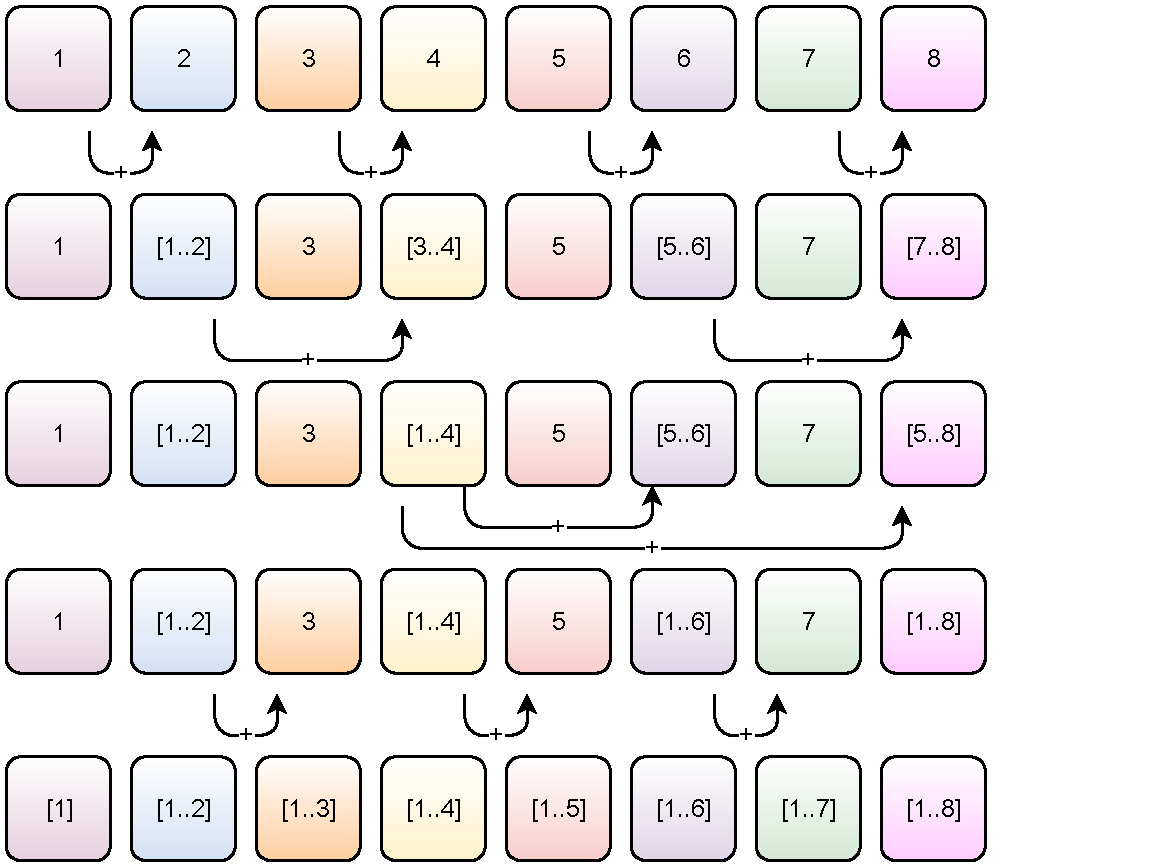
\includegraphics[width=0.8\textwidth]{./figures/oddeven.pdf}
  \caption{An example of parallelised \emph{inclusive scan} using the \emph{odd-even} algorithm, detailed in Algorithm~\ref{alg:parscan}}
  \label{fig:odd_even}
\end{center}
\end{figure}

\begin{algorithm}
  \caption{Odd-even style \emph{Scan} higher-order function with parallel execution.}
  \label{alg:parscan}

  \begin{algorithmic}
    \Function{ParScan}{$f, A$}
      \State{$level \Leftarrow 2$}

      \While{$level <= \|A\|$}
        \PFor{$l \in (level\ldots2 \times level\ldots\|A\|)$}
          \State{$A_l \Leftarrow$ \Call{$f$}{$A_l, A_{l - \frac{level}{2}}$}}
        \EndPFor
        \State{$level \Leftarrow 2 \times level$}
      \EndWhile

      \If{$level = \|A\|$}
      \State{$level \Leftarrow \frac{level}{2}$}
      \EndIf

      \While{$level > 1$}
      \PFor{$l \in (level + \frac{level}{2}\ldots2 \times level + \frac{level}{2}\ldots\|A\|)$}
          \State{$A_l \Leftarrow$ \Call{$f$}{$A_l, A_{l - \frac{level}{2}}$}}
        \EndPFor
        \State{$level \Leftarrow \frac{level}{2}$}
      \EndWhile

    \EndFunction
  \end{algorithmic}
\end{algorithm}

A parallel algorithm's \emph{cost} is defined as its asymptotic run-time multiplied by the required number of compute-units.


The \emph{odd-even} prefix sum algorithm can process a dataset of size $n$ in $O(\log n) + \frac{O(n)}{\|CU\|}$ stages of execution. This gives a cost of $O(\|CU\| \log n) + O(n)$.
Importantly, it is \emph{cost-optimal}, meaning that its cost is equal to that of the best-known sequential algorithm, when $\|CU\| = O(\frac{n}{\log n})$. This is an entirely reasonable assumption given large datasets and the comparatively low number of compute-units ($4-48$) present on commodity \ac{OpenCL} devices.

This discovery suggests that it is possible to increase the throughput of \verb|scan| tasks significantly, by scheduling them across massively parallel \ac{OpenCL} devices.

\subsection{Scatter}
The \verb|Scatter| primitive receives an input array $A$, an array of indices $I$, and an output array $B$. It updates $B$ such that $B_{I_i} \Leftarrow A_i$. Put otherwise, it inserts the value given at offset $i$ of $A$ into $B$, at the position given by the value at offset $i$ of $I$.

\verb|Scatter| is useful for reordering a collection or projecting a subset of an input dataset into an output dataset.

\begin{algorithm}
  \caption{\emph{Scatter} primitive with sequential execution.}
  \label{alg:seqscatter}

  \begin{algorithmic}
    \Function{SeqScatter}{$A, I, B$}
      \ForAll{$a_i \in A$}
      \State{$B_{I_i} \Leftarrow A_i$}
      \EndFor
    \EndFunction
  \end{algorithmic}
\end{algorithm}

\paragraph*{Permutation scatter}
It is important to draw attention to an important distinction in types of \verb|scatter| operation. \emph{Permutation Scatter} is defined as a scatter operation where all $i \in I$ are unique. Therefore, there are no two writes to the same destination in $B$. Other forms of \verb|scatter| increase complexity, as rules that state how to handle write collisions within the transaction must be introduced.

Luckily, for this project's needs we only need to analyse the simpler \emph{permutation scatter}. We can assume that no two writes to the same destination offset will occur.

\begin{figure}[h]
  \caption{\emph{Permutation Scatter} dependency graph}
  \label{fig:scatgraph1}
  \begin{center}
    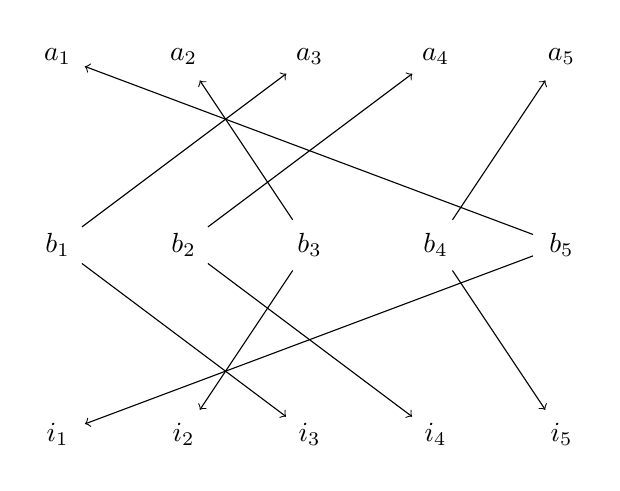
\begin{tikzpicture}
      [scale=.8,auto=left,every node/.style={circle}]

      \foreach \x in {1, 2, 3, 4, 5} {
        \node (a\x) at (2 * \x, 3) {$a_{\x}$};
        \node (b\x) at (2 * \x, 0) {$b_{\x}$};
        \node (i\x) at (2 * \x, -3){$i_{\x}$};
      }

      \foreach \s/\d in {1/5, 2/3, 3/1, 4/2, 5/4}{
        \draw[->] (b\d) -- (a\s);
        \draw[->] (b\d) -- (i\s);
      }

    \end{tikzpicture}
  \end{center}
\end{figure}
A data-dependency graph for a typical scatter operation is shown in Figure~\ref{fig:scatgraph1}.
At first, it may appear complicated. However, when nodes $b_i \in B$ are reordered by their data-source, a valid partitioning becomes clear. The result of this simplification is shown in Figure~\ref{fig:scatgraph2}.

\begin{figure}[h]
  \caption{\emph{Permutation Scatter} dependency graph, simplified.}
  \label{fig:scatgraph2}
  \begin{center}
    \begin{tikzpicture}
      [scale=.8,auto=left,every node/.style={circle}]

      \foreach \s/\d in {1/5, 2/3, 3/1, 4/2, 5/4}{
        \node (a\s) at (2 * \s, 2) {$a_{\s}$};
        \node (b\d) at (2 * \s, 0) {$b_{\d}$};
        \node (i\s) at (2 * \s, -2){$i_{\s}$};
        \draw[->] (b\d) -- (a\s);
        \draw[->] (b\d) -- (i\s);
      }
    \end{tikzpicture}
  \end{center}
\end{figure}

This suggests that \verb|scatter|, when using unique indices, is \emph{embarrassingly parallel}. Like \verb|map|, this produces an easy-to-understand parallel conversion, shown in Algorithm~\ref{alg:parscatter}.

\begin{algorithm}
  \caption{\emph{Permutation Scatter} primitive with parallel execution.}
  \label{alg:parscatter}

  \begin{algorithmic}
    \Function{ParScatter}{$A, I, B$}
      \PFor{$a_i \in A$}
      \State{$B_{I_i} \Leftarrow A_i$}
      \EndPFor
    \EndFunction
  \end{algorithmic}
\end{algorithm}

\paragraph*{Equivalent \ac{OpenCL} kernel design}
\begin{algorithm}
  \caption{\emph{Permutation Scatter} primitive in \ac{OpenCL} kernel form.}
  \label{alg:scatterkernel}
  \begin{algorithmic}
    \Function{ScatterKernel}{$A, I, B$}
      \State{$i \Leftarrow$ \Call{GetGlobalID}{}}
      \State{$B_{I_i} \Leftarrow A_i$}
    \EndFunction
  \end{algorithmic}
\end{algorithm}

The kernel design is simpler than that of \verb|map|, since function side-effects do not need to be included. It is presented in Algorithm~\ref{alg:scatterkernel}.

\subsection{Filter}
\verb|filter| is a higher-order function that applies a predicate function on elements of a dataset. It returns the subset of the input vector for which the predicate evaluates true. 

A sequential implementation of the primitive is shown in Algorithm~\ref{alg:seqfilter}.

\begin{algorithm}
  \caption{\emph{Filter} higher-order function with sequential execution.}
  \label{alg:seqfilter}

  \begin{algorithmic}
    \Function{SeqFilter}{$A, predicate$}
      \State{$Result \Leftarrow$ \verb|[ ]|}
      \ForAll{$a_i \in A$}
      \If{\Call{$predicate$}{$a_i$}}
      \State{\Call{Push}{$Result, a_i$}}
      \EndIf
      \EndFor
      \State{$A \Leftarrow Result$}
    \EndFunction
  \end{algorithmic}
\end{algorithm}

Checking the predicate is simple to do in parallel, since whether to keep each element depends only on the value of that element. However, producing and returning the subset is significantly more involved. Complication stems from the position of each kept item in the output array depending on the state of previous elements in the input vector.

\begin{figure}[h]
  \caption{\emph{Filter} dependency graph.}
  \label{fig:filtergraph}
  \begin{center}
    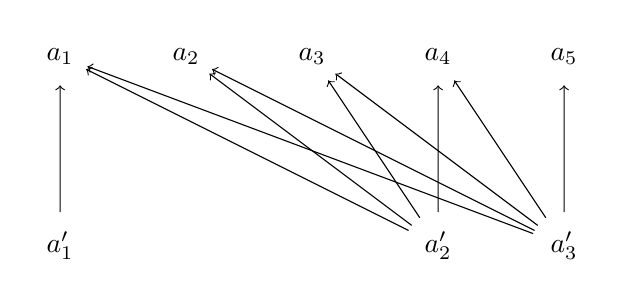
\begin{tikzpicture}
      [scale=.8,auto=left,every node/.style={circle}]

      \foreach \x in {1, 2, 3, 4, 5}{
        \node (a\x) at (2 * \x, 3) {$a_{\x}$};
      }

      \foreach \x/\y in {1/1, 4/2, 5/3}{
        \node (b\x) at (2 * \x, 0) {$a^\prime_{\y}$};
      }

      \draw[->] (b1) -- (a1);

      \draw[->] (b4) -- (a1);
      \draw[->] (b4) -- (a2);
      \draw[->] (b4) -- (a3);
      \draw[->] (b4) -- (a4);


      \draw[->] (b5) -- (a1);
      \draw[->] (b5) -- (a2);
      \draw[->] (b5) -- (a3);
      \draw[->] (b5) -- (a4);
      \draw[->] (b5) -- (a5);
    \end{tikzpicture}
  \end{center}
\end{figure}

The \verb|filter| operation is clearly not \emph{embarrassingly parallel}. However, there is no need to search for an involved parallel algorithm. We can construct an efficient \verb|filter| operation by reusing the previously defined parallel primitives, \verb|map|, \verb|scan|, and \verb|scatter|. This insight transforms a hard problem into one that is much easier to solve.

\paragraph*{Composing a parallel solution}
The first stage of producing a parallel \verb|filter| primitive is recognising the distinct data dependencies:
\begin{enumerate}
  \item Whether an element is kept.
  \item Where any kept element appears in the result.
  \item The total number of elements kept, since we cannot dynamically allocate memory.
\end{enumerate}

\subparagraph*{Identifying kept elements}
The information required by dependency $1$ can be obtained by performing a \verb|map| task on the dataset using the predicate function. The sole difference is that the result should be stored in a new buffer instead of overwriting the previous value.

Assuming we have an input vector $A$ and a newly created predicate buffer $P$, we now know that any $A_i$ should be kept if, and only if, $P_i$.

\subparagraph*{Knowing where to place kept elements}
Once we have produced a predicate buffer, via $1$, we can easily derive the destination of kept elements ($2$). If the predicate buffer is stored as a vector of bit-flags, the number of kept elements at point $P_i$ is equal to element $i$ of the prefix-summation of $P$. This connection is illustrated in Figure~\ref{fig:wheretoplace}

\begin{figure}[h]
\begin{center}
  \caption{Using prefix-sum to determine insertion points.}
  \label{fig:wheretoplace}

  $predicate$ = \verb|keep_if_even|
  \vskip 10pt
  \begin{tabular}{ | c | c | c | c | c | c |}
    \hline
    Input dataset   & 0 & 1 & 2 & 3 & 4 \\ \hline
    Presence buffer & 1 & 0 & 1 & 0 & 1 \\ \hline
    Prefix sum      & 1 & 1 & 2 & 2 & 3 \\ \hline
    Insertion point & 0 & - & 1 & - & 2 \\ \hline
  \end{tabular}
\end{center}
\end{figure}

The translation from prefix-summed buffer element to insertion point is just an off-by-one adjustment.
Furthermore, since \verb|map| followed by \verb|scan| is cost $O(n) + O(n) = O(n)$, we can obtain these insertion points \emph{cost-optimally}.

\subparagraph*{Counting the number of kept elements}
Following the calculation of dependencies $1$ and $2$, obtaining $3$ is trivial. It is simply the final element of the prefix-sum buffer. This can be retrieved by a single lookup after the other sub-problems have been solved.

\paragraph*{Complete solution}
By utilising \verb|map|, \verb|scan|, and a conditional-modified \verb|scatter|, \verb|filter| can be performed with cost $O(n) + O(n) + O(1) + O(n) = O(n)$. This is identical to the sequential algorithm presented earlier and is therefore \emph{cost-optimal}. Again, this suggests that \verb|filter| tasks can benefit from increased throughput when scheduled across multiple compute-units.

The combined process is demonstrated in Algorithm~\ref{alg:parfilter}.

\begin{algorithm}
  \caption{\emph{Filter} higher-order function with parallel execution, composed from other primitives.}
  \label{alg:parfilter}

  \begin{algorithmic}
    \Function{ParFilter}{$A, p$}
    \State{$P \Leftarrow$ \Call{ParMap}{$A, p$}}
    \State{$I \Leftarrow$ \Call{ParScan}{$P, +$}}
    \State{$B \Leftarrow$ \Call{Zeros}{$I_{\|I\|}$}}
    \PFor{$a_i \in A$}
      \If{$P_i$}
        \State{$B_{I_i - 1} \Leftarrow A_i$}
      \EndIf
    \EndPFor
    \State{$A \Leftarrow B$}
    \EndFunction
  \end{algorithmic}
\end{algorithm}

The parallel loop body is a modified version of the \verb|scatter| task. The divergence is that it only performs scattering if the predicate element is set.

\subsection{Count}
The \verb|count| function is very similar to the aforementioned \verb|filter| primitive.
Instead of returning the subset of a dataset that passes a predicate, it returns how many times the predicate was passed.

To avoid writing extra code providing counting functionality, we can re-use many components of the \verb|filter| implementation. Namely, the \verb|map| task that sets predicate bits for each element, followed by the \verb|scan| task to yield the number of kept elements. Reduction can be performed in  less work than a \verb|scan| primitive, as the intermediate values are not required. However it is asymptotically identical, therefore the \verb|scan| primitive can be reused to reduce developer workload.
Further work can include replacing this suboptimal lack of specialisation with a faster reduction task.


\subsection{Sort}
The project's sorting capability is provided by parallel \emph{bitonic mergesort}. Bitonic sorting utilises a sorting network of comparators to gradually produce a monotonically sorted result, from stages of increasing length bitonic sequences.

A simple implementation of bitonic mergesort, whereby single elements are compared and possibly swapped at each gate, can sort an input sequence of length $n$ with $O(n \log^2 n)$ cost. This is not cost-optimal as sequential sorting algorithms can perform the task in $O(n \log n)$ comparisons. However, sorting network based algorithms are suitable for \ac{SIMD} execution as the same sequence of comparisons will always occur, independent of the input elements' values.

The bitonic mergesort kernel, generated and dispatched for all RubiCL's \verb|sort| tasks, was adapted from sample code for sorting provided within the \ac{AMD} APP SDK.
